\section{k-Means}
\label{mainsec:kmeans}
\textit{Alexander Baumgärtner, Robert Brylka}

%Hintergrund (Motivation/Geschichtliches)
Der Begriff k-Means bezeichnet einen Clustering-Algorithmus von Stuart P. Lloyd \cite{Lloyd}, der 1957 entwickelt und erst 1982 in einer Fachzeitschrift veröffentlicht wurde. Unter Clustering versteht man hierbei die Gruppierung von Daten mit ähnlichen Eigenschaften in gleiche Klassen. Die Berechnung der optimalen Lösung eines solchen Klassifikationsproblems ist NP-schwer \cite{kMeansNPhard}. Aus diesem Grund sind Heuristiken wie k-Means hilfreich, um dennoch in angemessener Zeit eine akzeptable Lösung zu finden.
Solche Verfahren gehören zur Obergruppe des unüberwachten Lernens, bei denen die Trainingsphase durchlaufen wird, ohne dass 
bekannt ist, welche Daten zu welcher Klasse gehören.

\subsection{Funktionsweise des Klassifikators (Allgemein)} \label{subsec:kMeansFunktionsweise}
K-Means segmentiert eine Datenmenge in \emph{k} verschiedene Cluster, indem \emph{k} Cluster-Zentren berechnet werden und ein zu klassifizierendes Objekt immer dem nächstgelegenen Cluster-Zentrum zugeordnet wird. Dazu ist es jedoch notwendig, dass die Daten numerisch vorhanden sind. Textuelle Daten kann k-Means nicht verarbeiten.
Der Algorithmus arbeitet schnell und effizient, findet jedoch im besten Fall nur ein lokales Optimum. Unter bestimmten Bedingungen konvergiert der k-Means Algorithmus jedoch nicht einmal zum lokalen Optimum \cite{kMeansMinimum}. Aus diesem Grund ist es hilfreich, die Lernphase mehrere Male zu wiederholen und anschließend den Klassifikator mit der geringsten Fehlerquote zu verwenden.  

Der Algorithmus läuft folgendermaßen ab \cite{Marsland}:
\begin{itemize}

\item \emph{Initialisierung:} Es wird ein geeigneter Wert \emph{k} für die Anzahl der zu findenden Cluster gewählt.
Anschließend werden \emph{k} zufällige Positionen im Eingaberaum bestimmt und jeweils als Cluster-Zentren festgelegt (siehe \autoref{fig:lernenEinfach} oben links).
\item \emph{Training:} Für jeden Datenpunkt wird der Abstand zu allen Cluster-Zentren berechnet und anschließend der Datenpunkt dem Zentrum mit dem geringsten Abstand zugeordnet. 
Danach wird jedes Cluster-Zentrum in den Schwerpunkt aller ihm zugeordneten Punkte verschoben.
Der gesamte Lernvorgang wiederholt sich solange, bis sich die Position der Cluster-Zentren nicht mehr verändert. 
Ein Beispiel für einen Trainingsvorgang ist in \autoref{fig:lernenEinfach} dargestellt.
\item \emph{Benutzung:} Um das passende Cluster zu einen Datenpunkt zu bestimmen, wird dessen Abstand zu allen Cluster-Zentren berechnet. Das Cluster, dessen Zentrum den geringsten Abstand hat, wird dem Datenpunkt zugeordnet. In \autoref{fig:lernenEinfach} unten rechts ist  eine solche Bestimmung anhand der zuvor berechneten Cluster-Zentren dargestellt. Die Zugehörigkeit beliebiger Objekte zu den jeweiligen Cluster-Zentren ist durch Trennlinien markiert.
\end{itemize}


\begin{figure*}[htbp]
    \centering
   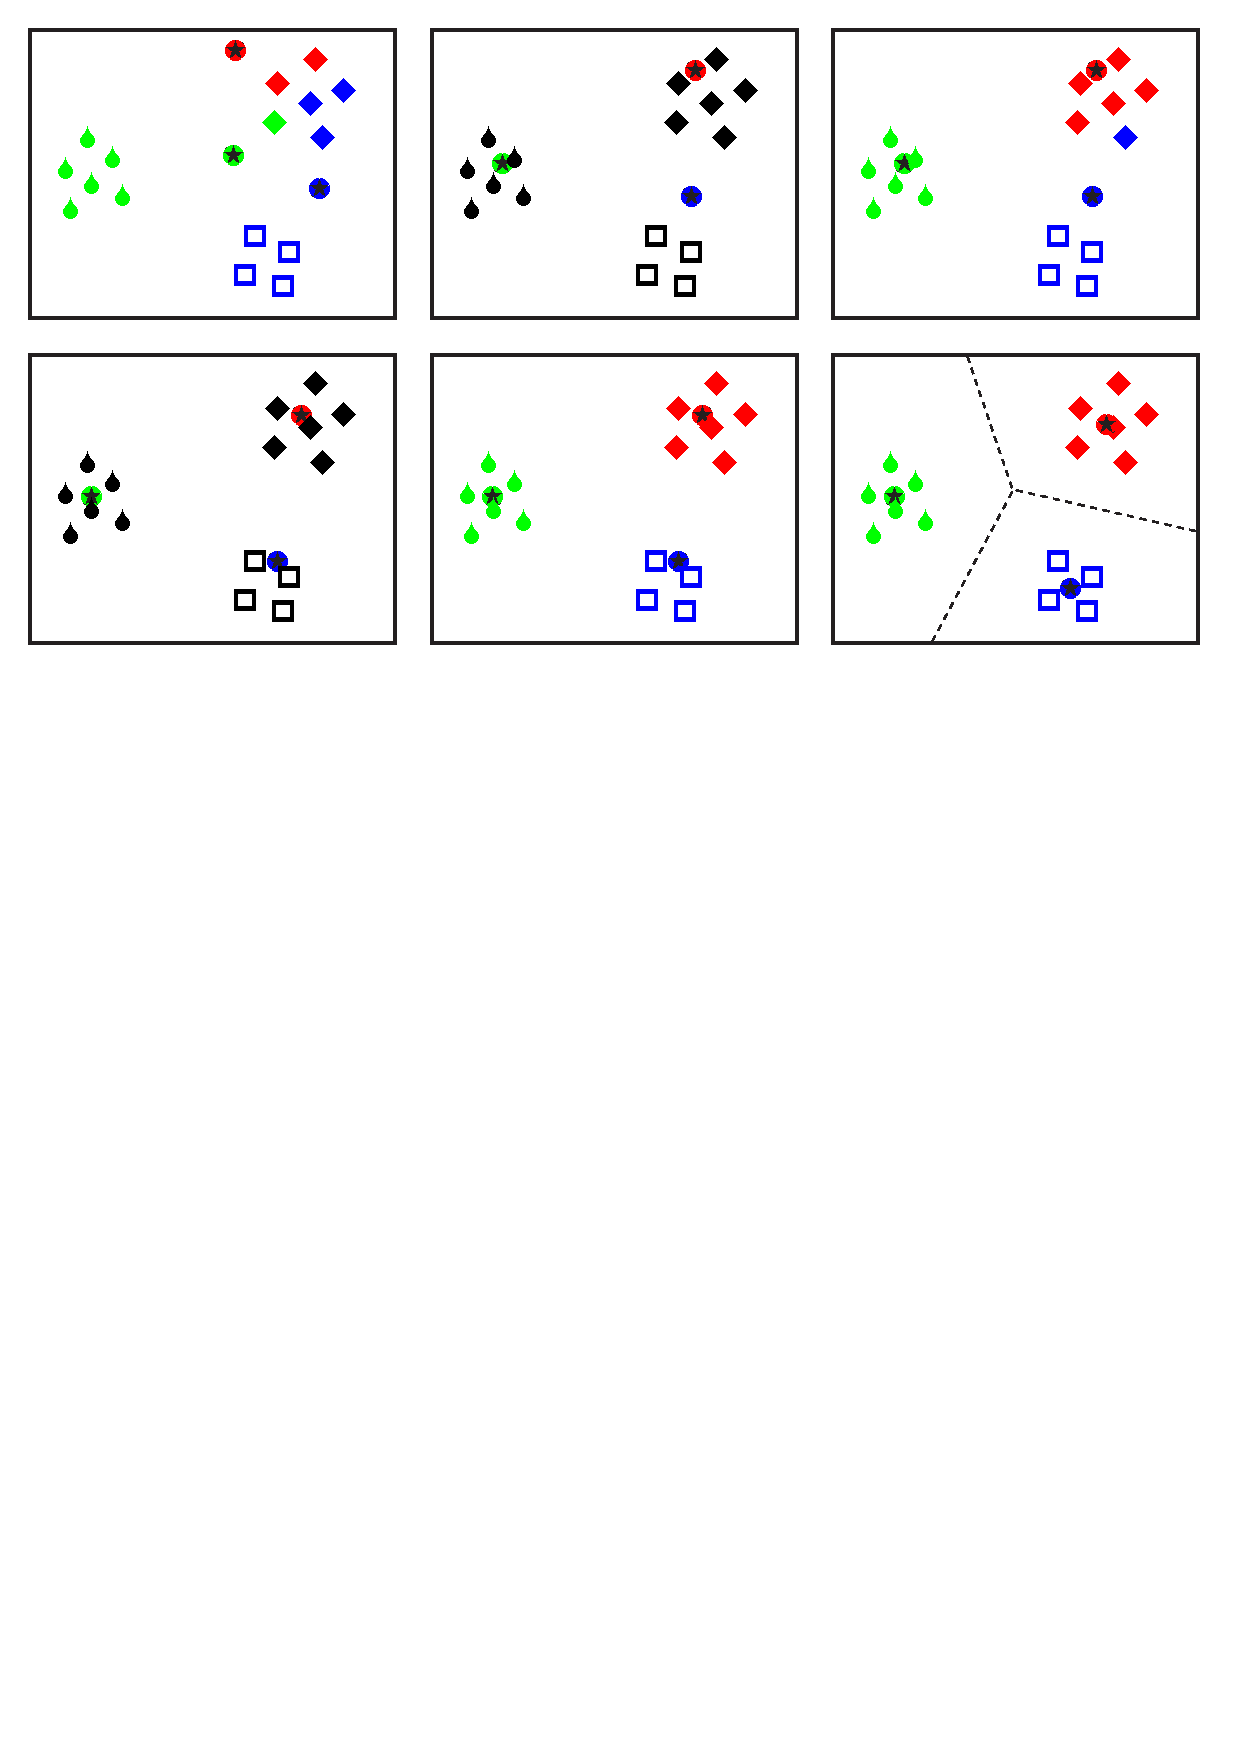
\includegraphics[width=.95\textwidth]{kmeans/lernenEinfach.pdf}
\caption{Trainingsphase beim k-Means Algorithmus}
\label{fig:lernenEinfach}
\end{figure*}

%Zu Beginn der Lernphase des Algorithmus wird ein Wert für \emph{k} festgelegt und anschließend werden \emph{k} zufällige Positionen im Eingaberaum als Cluster-Zentren gesetzt (siehe \autoref{fig:lernenEinfach}, oben links). Danach wird jedes Zentrum in den Schwerpunkt der ihm zugeordneten Objekte verschoben, sodass der Abstand zwischen Cluster-Zentrum und zugeordneten Objekten minimal wird. Diese Verschiebungen werden solange wiederholt, bis sich die Cluster-Zentren nicht mehr bewegen. 
%Um nun zu einem Objekt das passende Cluster-Zentrum zuzuordnen, wird der Abstand zwischen Objekt und den Cluster-Zentren berechnet. Das Objekt wird nun dem Cluster-Zentrum mit dem geringsten Abstand zugeordnet. 


K-Means benötigt in der Regel beim Lernen mehr Zeit als bei der Benutzung, da im ersten Fall die Cluster-Zentren unter Umständen oft verschoben werden und nach jeder Verschiebung erneut die Abstände zu allen dem Zentrum zugeordneten Punkten berechnet werden müssen. Bei der Benutzung hingegen genügt es, nur die Abstände des zu klassifizierenden Punkts zu allen Cluster-Zentren zu berechnen, um das passende Cluster zu bestimmen. Der Algorithmus arbeitet jedoch
in beiden Phasen verhältnismäßig schnell, da immer nur 
der -- rechnerisch wenig aufwändige -- euklidische Abstand ermittelt wird.
Weiterhin ist festzuhalten, dass k-Means anfällig für Ausreißer ist, d.h. einzelne falsche Daten wie beispielsweise Messfehler können ein Cluster-Zentrum unter Umständen stark verschieben.

Es existieren weiterhin einige Variationen des Basis-Algorithmus, mit dem dieser weiter optimiert werden kann. Dazu gehört etwa ein vorzeitiger Abbruch des Lernens, wenn eine festgelegte Maximalzahl von Iterationen erreicht wurde. Mit dem k-Means++ Algorithmus \cite{kMeans++} kann die Dauer der Lernphase verkürzt und die Fehlerrate bei der Benutzung gesenkt werden. Dieser Algorithmus wird in der Initialisierungsphase zur Bestimmung der Startpositionen der Cluster-Zentren verwendet. Dabei werden die Startpositionen der Cluster-Zentren nicht wie beim ursprünglichen Algorithmus zufällig gewählt, sondern wie folgt aus allen Eingabedaten $X$ bestimmt:
\begin{itemize}
\item Als erstes Cluster-Zentrum wird zufällig gleichverteilt ein Punkt aus $X$ gewählt.
\item Ein weiteres Cluster-Zentrum wird folgendermaßen ermittelt: 
\begin{itemize}
\item Die Entfernung $D(x)$ von allen Datenpunkten $x$ zu dem Cluster-Zentrum mit dem jeweils geringsten Abstand wird berechnet. 
\item Als neues Cluster-Zentrum wird zufällig ein Punkt aus den Eingabedaten bestimmt, wobei jeder Punkt $x$ mit der Wahrscheinlichkeit $\frac{ D(x)^{2} }{\sum\nolimits_{x \in X}D(x)^{2}}$ gewählt wird.
\end{itemize}
\item Der vorherige Schritt wird solange wiederholt, bis die gewünschte Menge an Cluster-Zentren berechnet ist.
\item Anschließend wird mit der Trainingsphase des ursprünglichen k-Means Algorithmus fortgefahren.
\end{itemize}


\subsection{Anwendung auf Projekt}
Selbstverständlich wird versucht, die Fehlerquote bei der Gestenerkennung zu minimieren. Dabei ist es jedoch besonders wichtig, dass das Grundrauschen nicht fälschlicherweise als Geste erkannt wird. In einem solchen Fall würde es zu einer ungewollten Steuerung ohne Bewegung des Benutzers kommen.
%, da die Aktion der irrtümlich erkannten Geste ausgeführt wird.
Ebenso sollten andere Bewegungen beim Bedienen des Rechners wie etwa das Tippen auf der Tastatur oder eine Bewegung der Maus möglichst nicht als Geste erkannt werden.
Weniger bedeutend ist es hingegen, wenn umgekehrt eine Geste als Grundrauschen klassifiziert wird. In diesem Fall wird der Anwender die Geste wiederholen, bis diese erkannt und die zugeordnete Aktion ausgeführt wird.

Zur besseren Erkennung der Gesten ist es notwendig, die Rohdaten vor der Klassifikation zu filtern. Diese Vorverarbeitung wird in \autoref{subsubsec:Datenaufbereitung} näher beschrieben.

Zur Erkennung des Grundrauschens gibt es zwei Möglichkeiten: Entweder können eine oder mehrere weitere Klassen eingeführt werden, die für das Grundrauschen stehen. Oder der maximale Abstand von Geste und Cluster-Zentrum wird auf einen Maximalwert begrenzt, sodass
eine Aufnahme als Grundrauschen klassifiziert wird, wenn der Abstand zu allen Cluster-Zentren den Maximalwert überschreitet.
%In ersten Tests zeigte sich, dass eine Erkennung des Grundrauschens mit einer zusätzlichen Klasse zuverlässig funktioniert. Daher wurde die zweite Variante eines maximalen Abstands zu den Cluster-Zentren -- die zusätzlichen Aufwand für die Anpassung der verwendeten Bibliothek sowie zur Ermittlung dieses Maximalwerts verursacht hätte -- nicht weiter verfolgt.


\subsubsection{Datenaufbereitung}\label{subsubsec:Datenaufbereitung}
%Für die Klassifikation mit dem k-Means Algorithmus wurde die Anzahl der Frames einer Aufnahme von dem ursprünglichen Wert 32 auf 48
Für die Klassifikation mit dem k-Means Algorithmus wurden nicht -- wie ursprünglich vorgesehen -- 32 Frames, sondern stattdessen 48 Frames pro Aufnahme gespeichert. 
Diese Anzahl wurde angepasst, da sich gezeigt hat, dass manche Gesten nicht in die 32 Frames hineinpassen. Die Datenaufbereitung kann daher mit 48 Frames besser realisiert werden.
%Diese Anzahl wurde angepasst, da sich herausgestellt hat, dass die Datenaufbereitung so besser realisieren werden kann.
Ein einzelner Frame besteht jedoch weiterhin aus 64 Lautstärkewerten.
%Die Rohdaten einer Aufnahme bestehen aus 48 Frames, die jeweils 64 Lautstärkewerte beinhalten. 
Jeder Lautstärkewert entspricht dabei der Intensität des Tonsignals in dem jeweiligen Frequenzbereich, welche mithilfe der schnellen Fourier-Transformation (\emph{FFT}) \cite{fftMathebuch} berechnet wurde. Eine einzelne Aufnahme besteht daher aus $48 \cdot 64 = 3072$ Dimensionen.  Da hochdimensionale Eingabedaten bei Clustering-Verfahren oft schlechte Ergebnisse liefern \cite{kMeansHighDimensions}, ist es notwendig, bei der Datenaufbereitung die Dimension der Eingabedaten zu reduzieren.  Erste Tests mit nicht aufbereiteten 
%2048-dimensionalen 
Eingabedaten lieferten eine korrekte Erkennungsrate von etwa 25 bis 30 Prozent bei 7 Klassen (6 Gesten sowie Grundrauschen ohne Geste). Lediglich das Grundrauschen kann so einigermaßen zuverlässig erkannt werden, eine korrekte Unterscheidung der einzelnen Gesten ist jedoch nicht möglich. Dies zeigt deutlich die Notwendigkeit einer Datenaufbereitung.

Bei allen Aufnahmen der Gesten befindet sich die Amplitude bei 18,5 kHz, da dies der abgespielten Referenzfrequenz entspricht. Durch den Doppler-Effekt entstehen bei der Ausführung der Gesten zusätzliche lokale Maxima, die Amplitude verschiebt sich jedoch nicht.
%Bei der Analyse der Frequenzspektren der einzelnen Gesten lassen sich folgende Besonderheiten erkennen:
Die Analyse der Frequenzspektren der einzelnen Gesten zeigt folgende Besonderheiten:

\begin{figure*}[htbp]
    \centering
   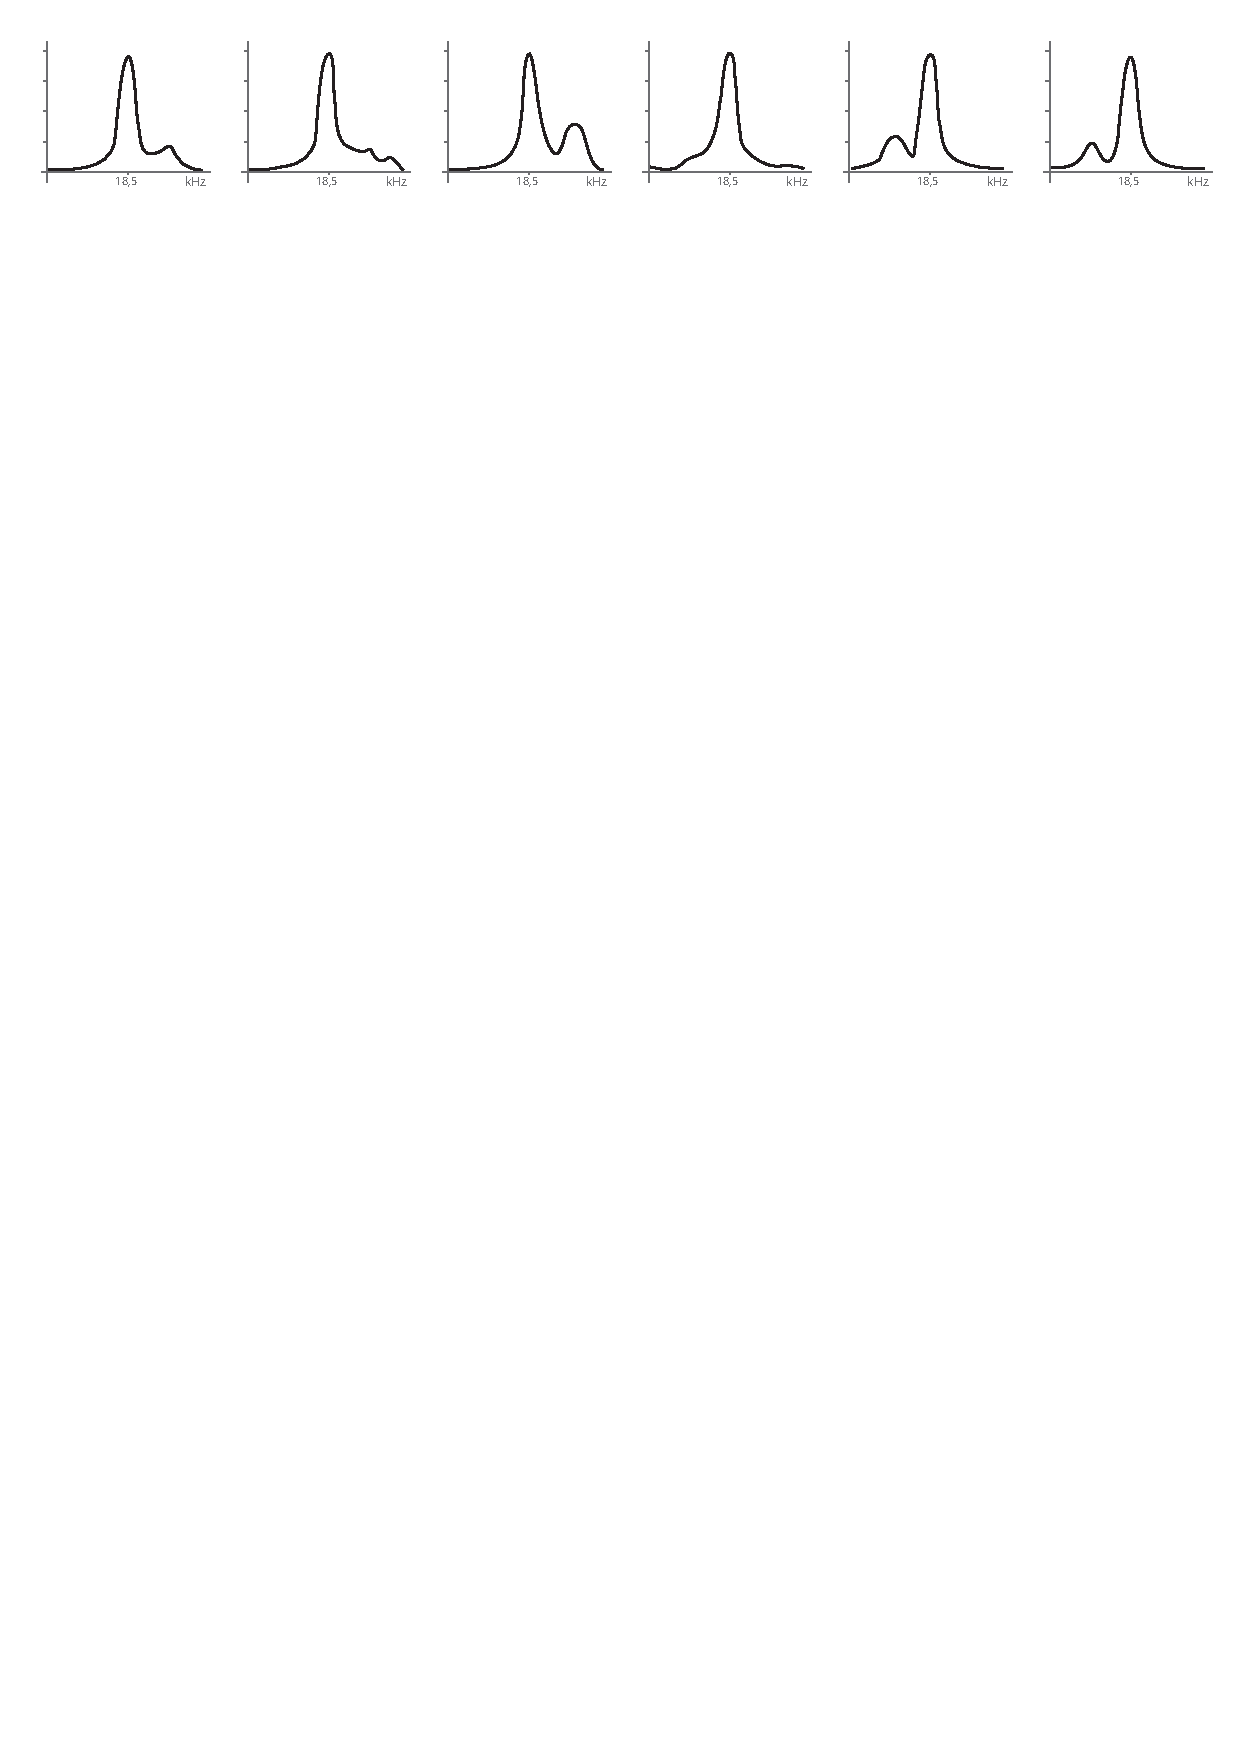
\includegraphics[width=\textwidth]{kmeans/Geste0.pdf}
\caption{Frequenzspektrum der Geste \ac{RLO}}
\label{fig:kMeansGeste0}
\end{figure*}

\begin{figure*}[htbp]
    \centering
   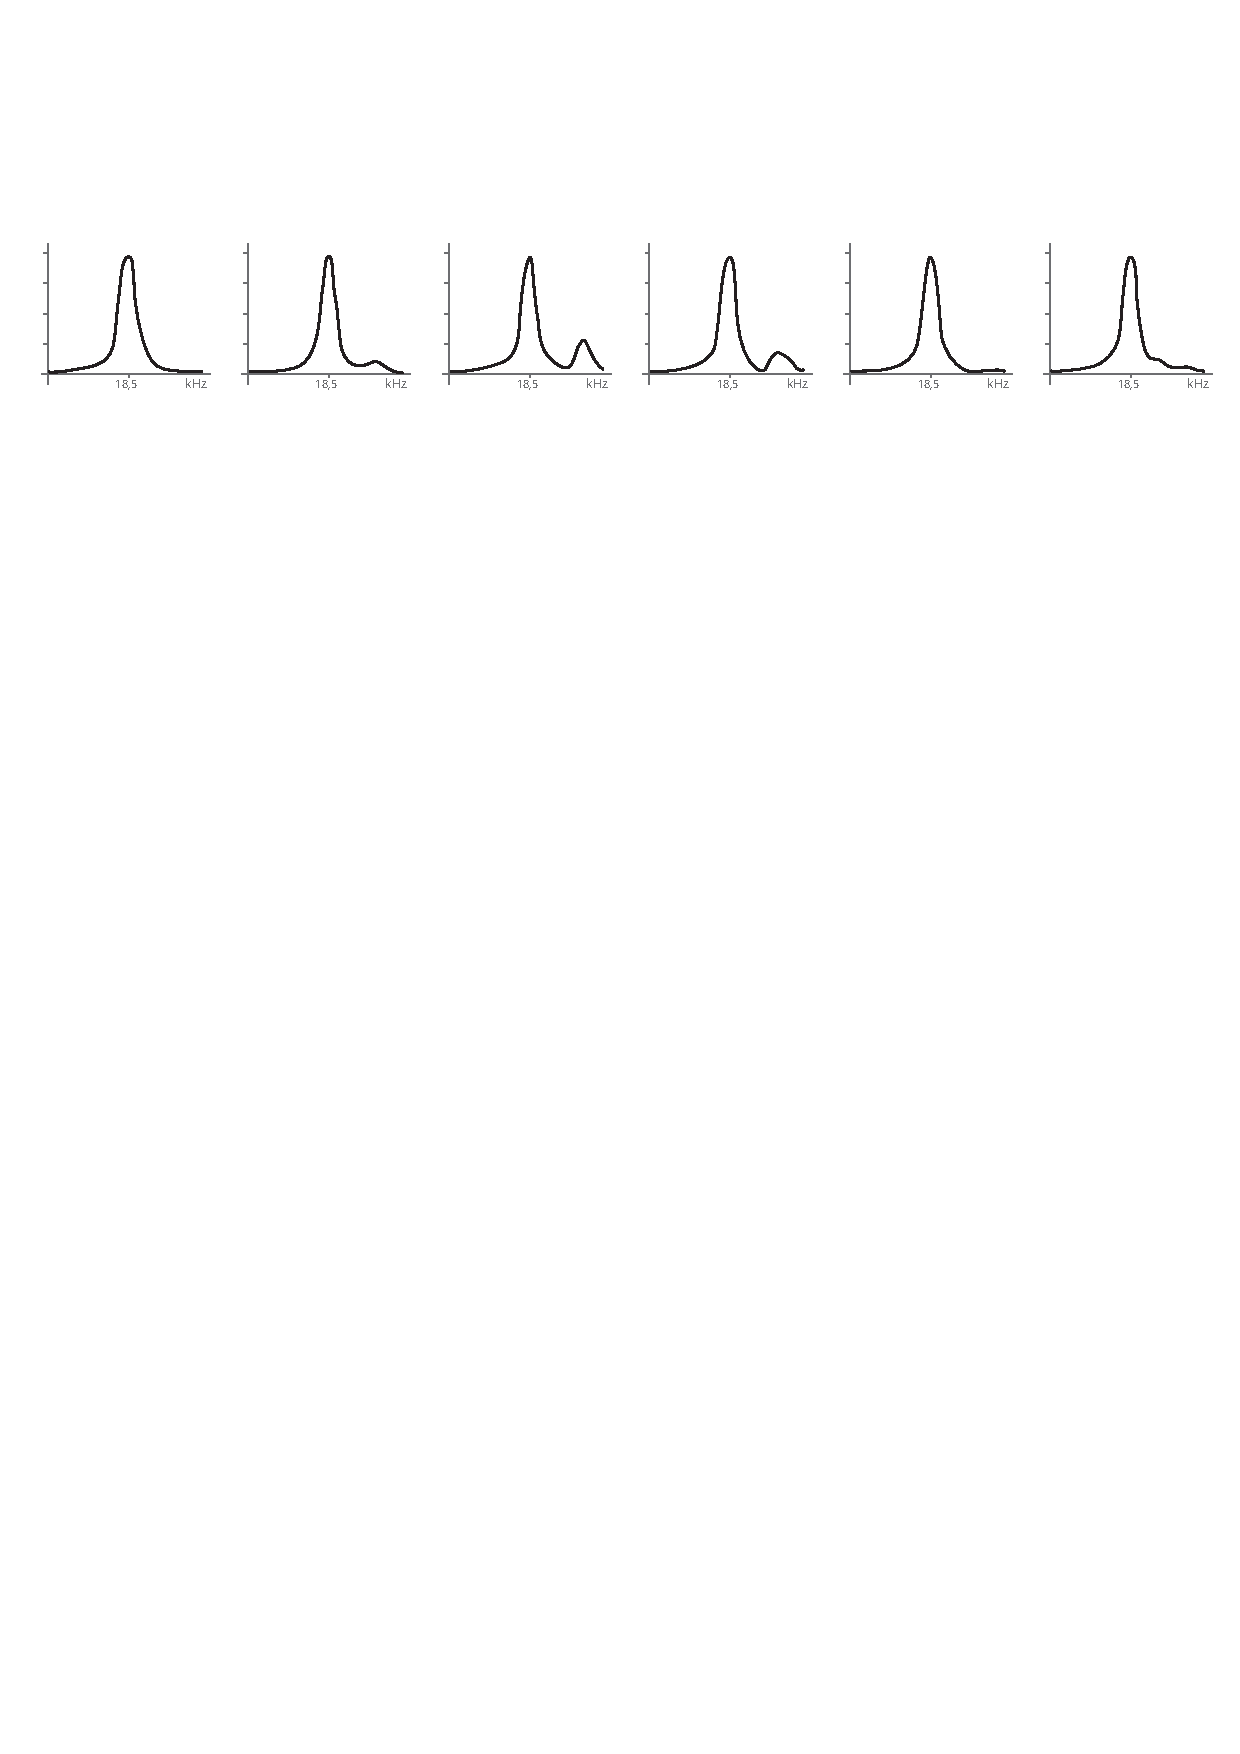
\includegraphics[width=\textwidth]{kmeans/Geste1.pdf}
\caption{Frequenzspektrum der Geste \ac{TBO}}
\label{fig:kMeansGeste1}
\end{figure*}

\begin{figure*}[htbp]
    \centering
   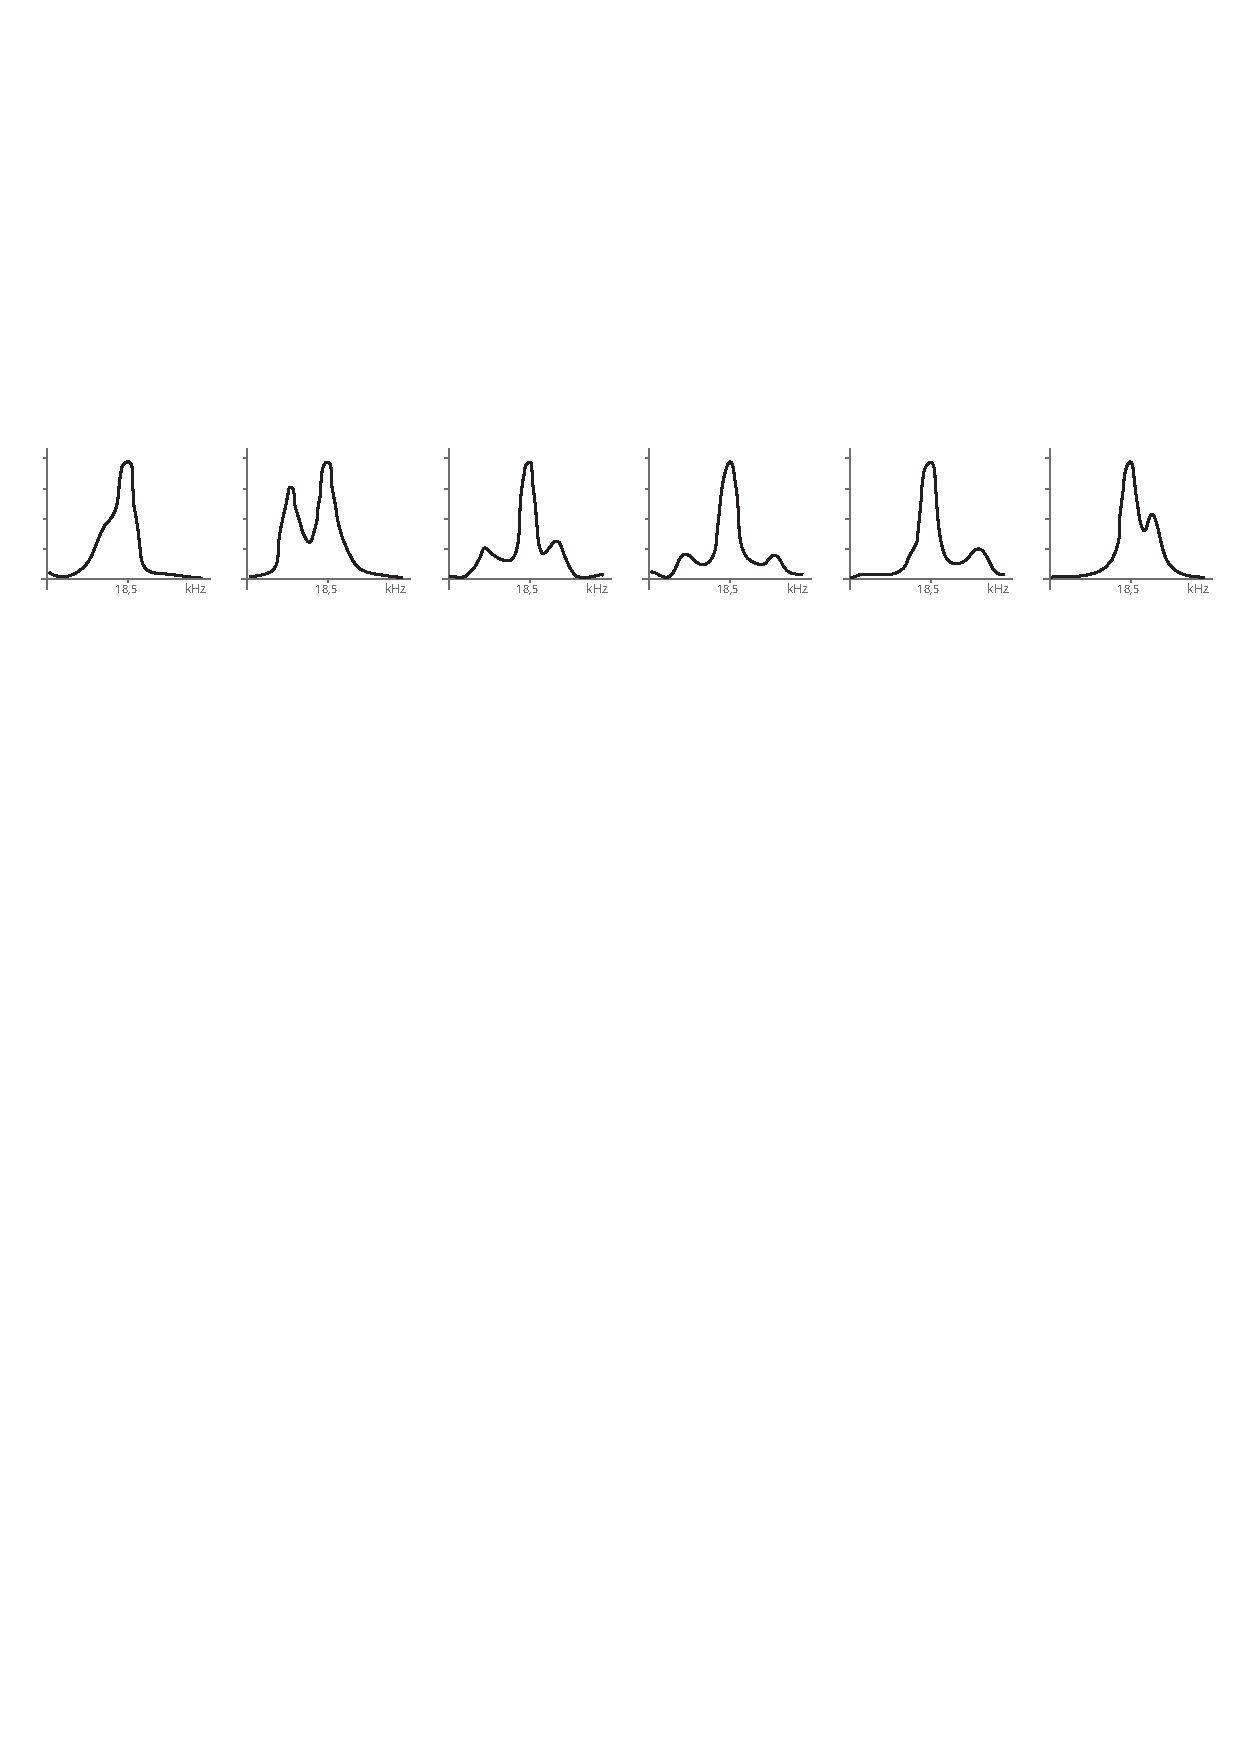
\includegraphics[width=\textwidth]{kmeans/Geste2.pdf}
\caption{Frequenzspektrum der Geste \ac{OT} (erste Hälfte)}
\label{fig:kMeansGeste2}
\end{figure*}

\begin{figure*}[htbp]
    \centering
   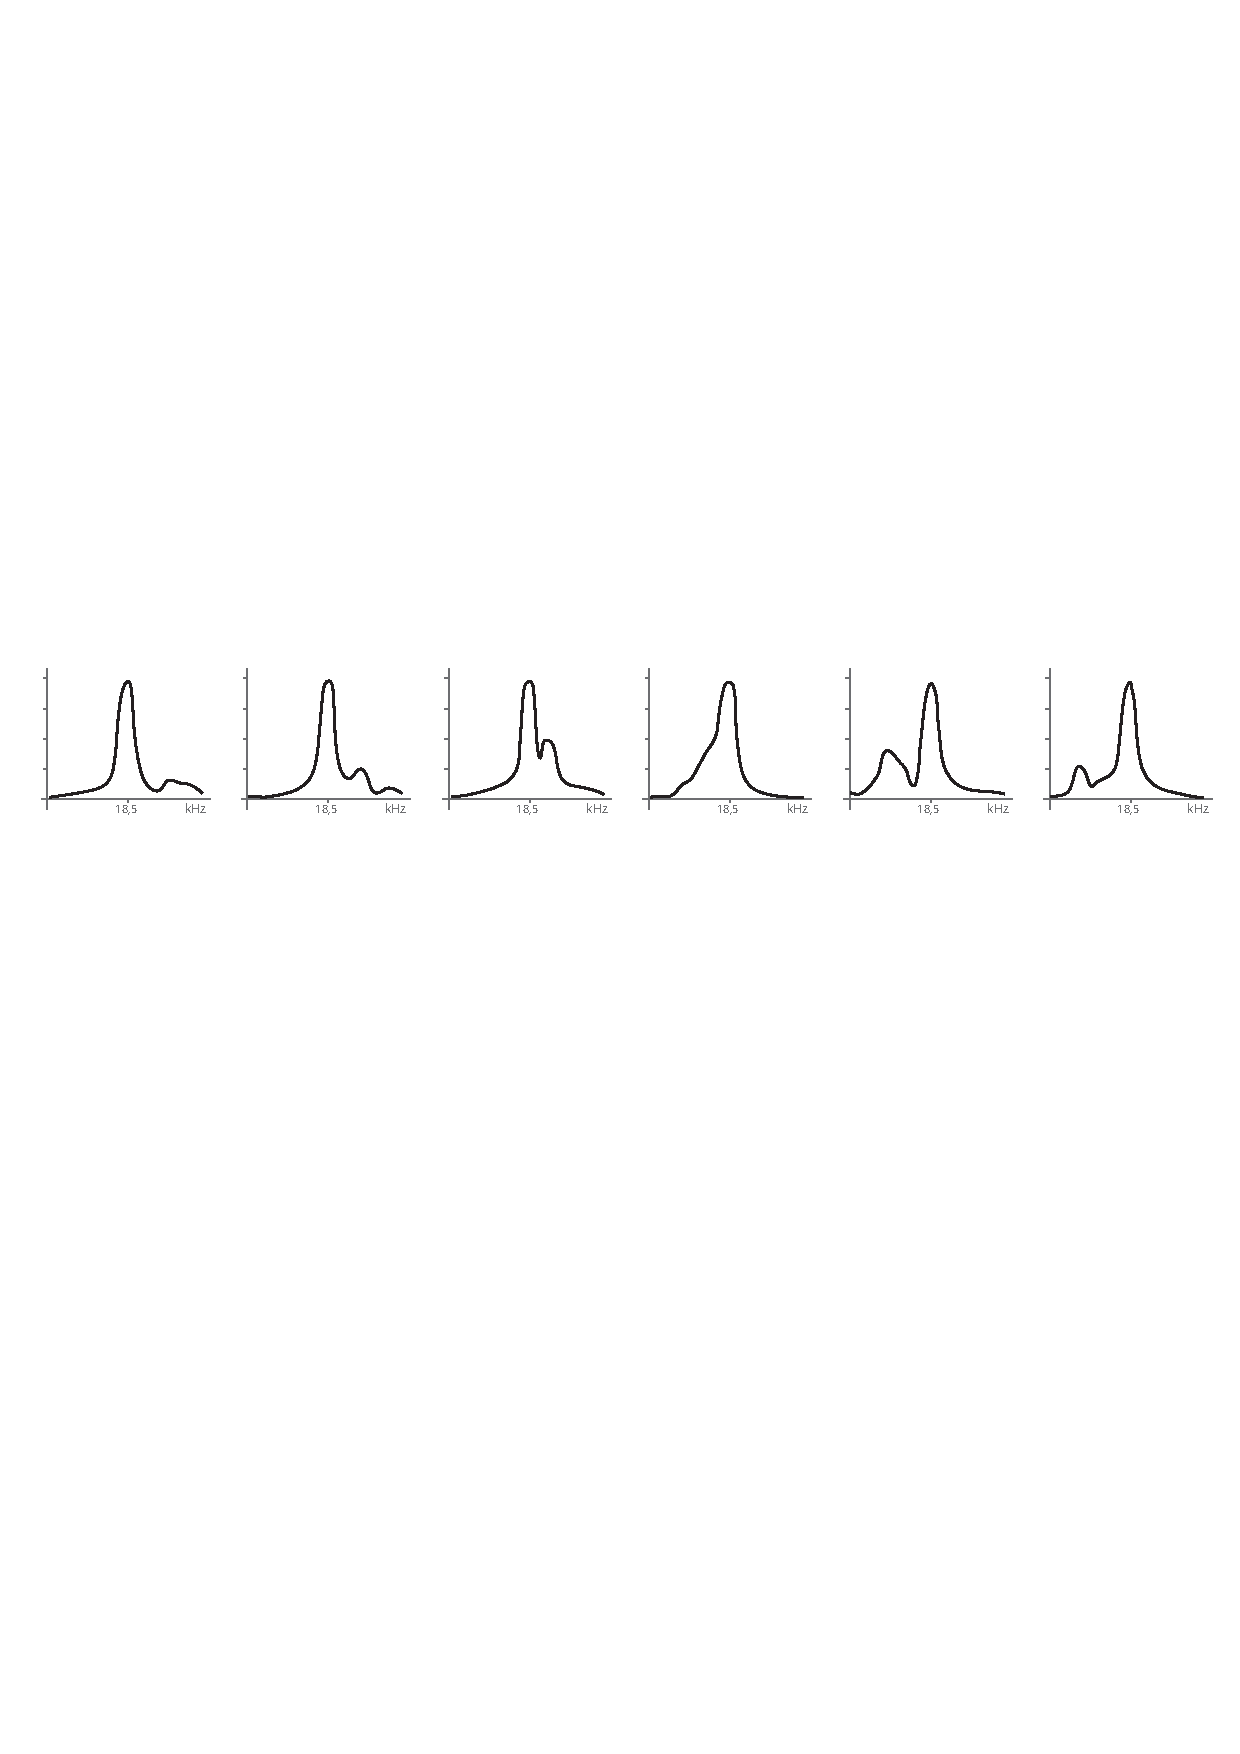
\includegraphics[width=\textwidth]{kmeans/Geste3.pdf}
\caption{Frequenzspektrum der Geste \ac{SPO}}
\label{fig:kMeansGeste3}
\end{figure*}

\begin{figure*}[htbp]
    \centering
   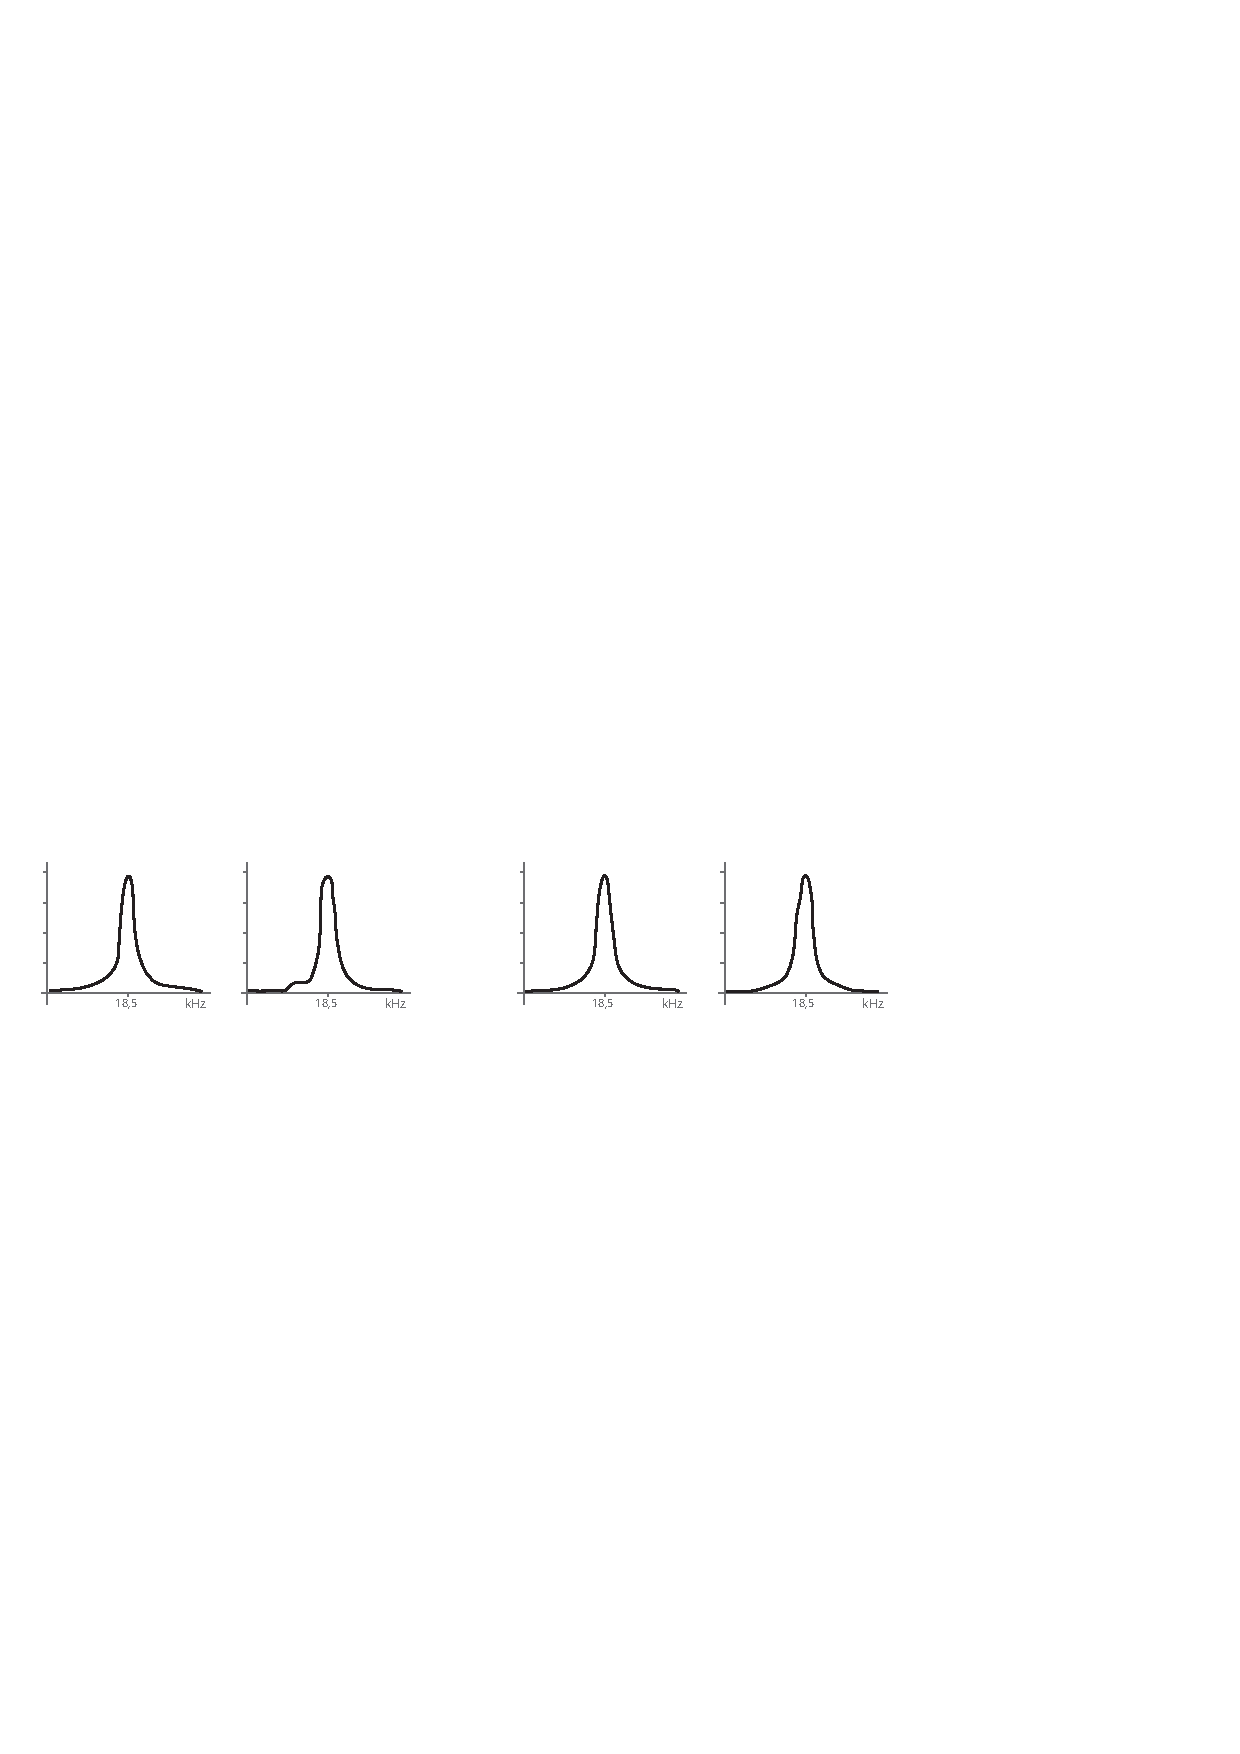
\includegraphics[width=\textwidth]{kmeans/Gesten6und7.pdf}
\caption{Frequenzspektrum der Gesten \ac{BNS} (links) und \ac{BNN} (rechts)}
\label{fig:kMeansGesten6und7}
\end{figure*}


\begin{itemize}
%0: Right-To-Left-One-Hand
\item \ac{RLO} (\autoref{fig:kMeansGeste0}): Bei dieser Geste tritt zu Beginn ein lokales Maximum im Frequenzbereich oberhalb der Amplitude auf. Anschließend erhöht sich der Wert dieses Maximums und wandert im weiteren Verlauf in den Frequenzbereich unterhalb der Amplitude. Zuletzt verringert sich der Wert des Maximums wieder.

%1: Top-To-Bottom-One-Hand
\item \ac{TBO} (\autoref{fig:kMeansGeste1}): Zu Beginn der Geste bildet sich ein lokales Maximum im Frequenzbereich oberhalb der Amplitude. Der Wert dieses Maximums erhöht sich im weiteren Verlauf und nimmt gegen Ende wieder ab.

%2: Opposed-With-Two-Hands
\item \ac{OT} (\autoref{fig:kMeansGeste2}): Durch die Bewegung mit zwei Händen kommt es zu einer komplexeren Veränderung des Tonsignals als bei den Gesten mit einer Hand. Zu Beginn der Geste entsteht durch das Bewegen der einen Hand vom Bildschirm weg ein lokales Maximum im Frequenzbereich unterhalb der Amplitude (Frame 2). Wenn sich anschließend beide Hände auf gleicher Höhe befinden, sind zwei lokale Maxima jeweils oberhalb und unterhalb der Amplitude zu erkennen (Frames 3 und 4). 
Danach kommt es durch die Bewegung der anderen Hand in Richtung des Bildschirms zu einem lokalen Maximum oberhalb der Amplitude (Frames 5 und 6).
Diese Bewegungsfolge sowie die entsprechenden Veränderungen des Frequenzspektrums wiederholen noch einmal in der gleichen Reihenfolge.
%Wenn die Hand wieder vom Bildschirm wegbewegt wird (Frame 9), entsteht wieder ein lokales Maximum unterhalb der Amplitude. Wenn sich beide Hände wieder auf gleicher Höhe befinden, sind wieder zwei lokale Maxima oberhalb und unterhalb der Amplitude zu erkennen (Frame 11).  Zuletzt entsteht durch die Bewegung in Richtung des Bildschirms wieder ein lokales Maximum oberhalb der Amplitude. (Frame 13)
%Wenn die Hand wieder vom Bildschirm wegbewegt wird (Frame 9), entsteht wieder ein lokales Maximum unterhalb der Amplitude. Wenn sich beide Hände wieder auf gleicher Höhe befinden, sind wieder zwei lokale Maxima oberhalb und unterhalb der Amplitude zu erkennen (Frame 11).  Zuletzt entsteht durch die Bewegung in Richtung des Bildschirms wieder ein lokales Maximum oberhalb der Amplitude. (Frame 13)

%3: Single-Push-One-Hand
\item \ac{SPO} (\autoref{fig:kMeansGeste3}): Ebenso wie bei der Geste \ac{RLO} kommt es zu einer Verschiebung des lokalen Maximums vom Frequenzbereich oberhalb der Amplitude zum Frequenzbereich unterhalb der Amplitude.

%4: Double-Push-One-Hand
\item \ac{DPO}: Hierbei kommt es zweimal hintereinander zu den bei Geste \ac{SPO} beschriebenen Effekten.

%5: Rotate-One-Hand
\item \ac{RO} Bei dieser Geste sind innerhalb des betrachteten Frequenzspektrums keine Unterschiede zum Hintergrundrauschen (\ac{BNS} und \ac{BNN}) zu erkennen.

%6+7: Background-Noise-Silent und Background-Noise-Noisy
\item \ac{BNS} und \ac{BNN} (\autoref{fig:kMeansGesten6und7}): Bei diesen beiden Klassen für das Hintergrundrauschen sind neben der Amplitude bei 18,5 kHz keine weiteren Peaks vorhanden. Durch die Ungenauigkeit von Mikrofon und Lautsprecher entstehen lediglich geringe, kaum sichtbare Schwankungen der Lautstärkewerte. Zwischen dem Hintergrundrauschen in lauter und in leiser Umgebung sind innerhalb des betrachteten Frequenzbereichs keine Unterschiede zu erkennen.

\end{itemize}

Die Klassifizierung der Geste \ac{RLO} wurde nicht weiter verfolgt, da sie nicht zuverlässig von Geste \ac{SPO} unterschieden werden kann. Ebenso wird Geste \ac{RO} nicht weiter betrachtet, da sich diese nicht vom Hintergrundrauschen unterscheiden lässt.

\begin{figure*}[htbp]
    \centering
   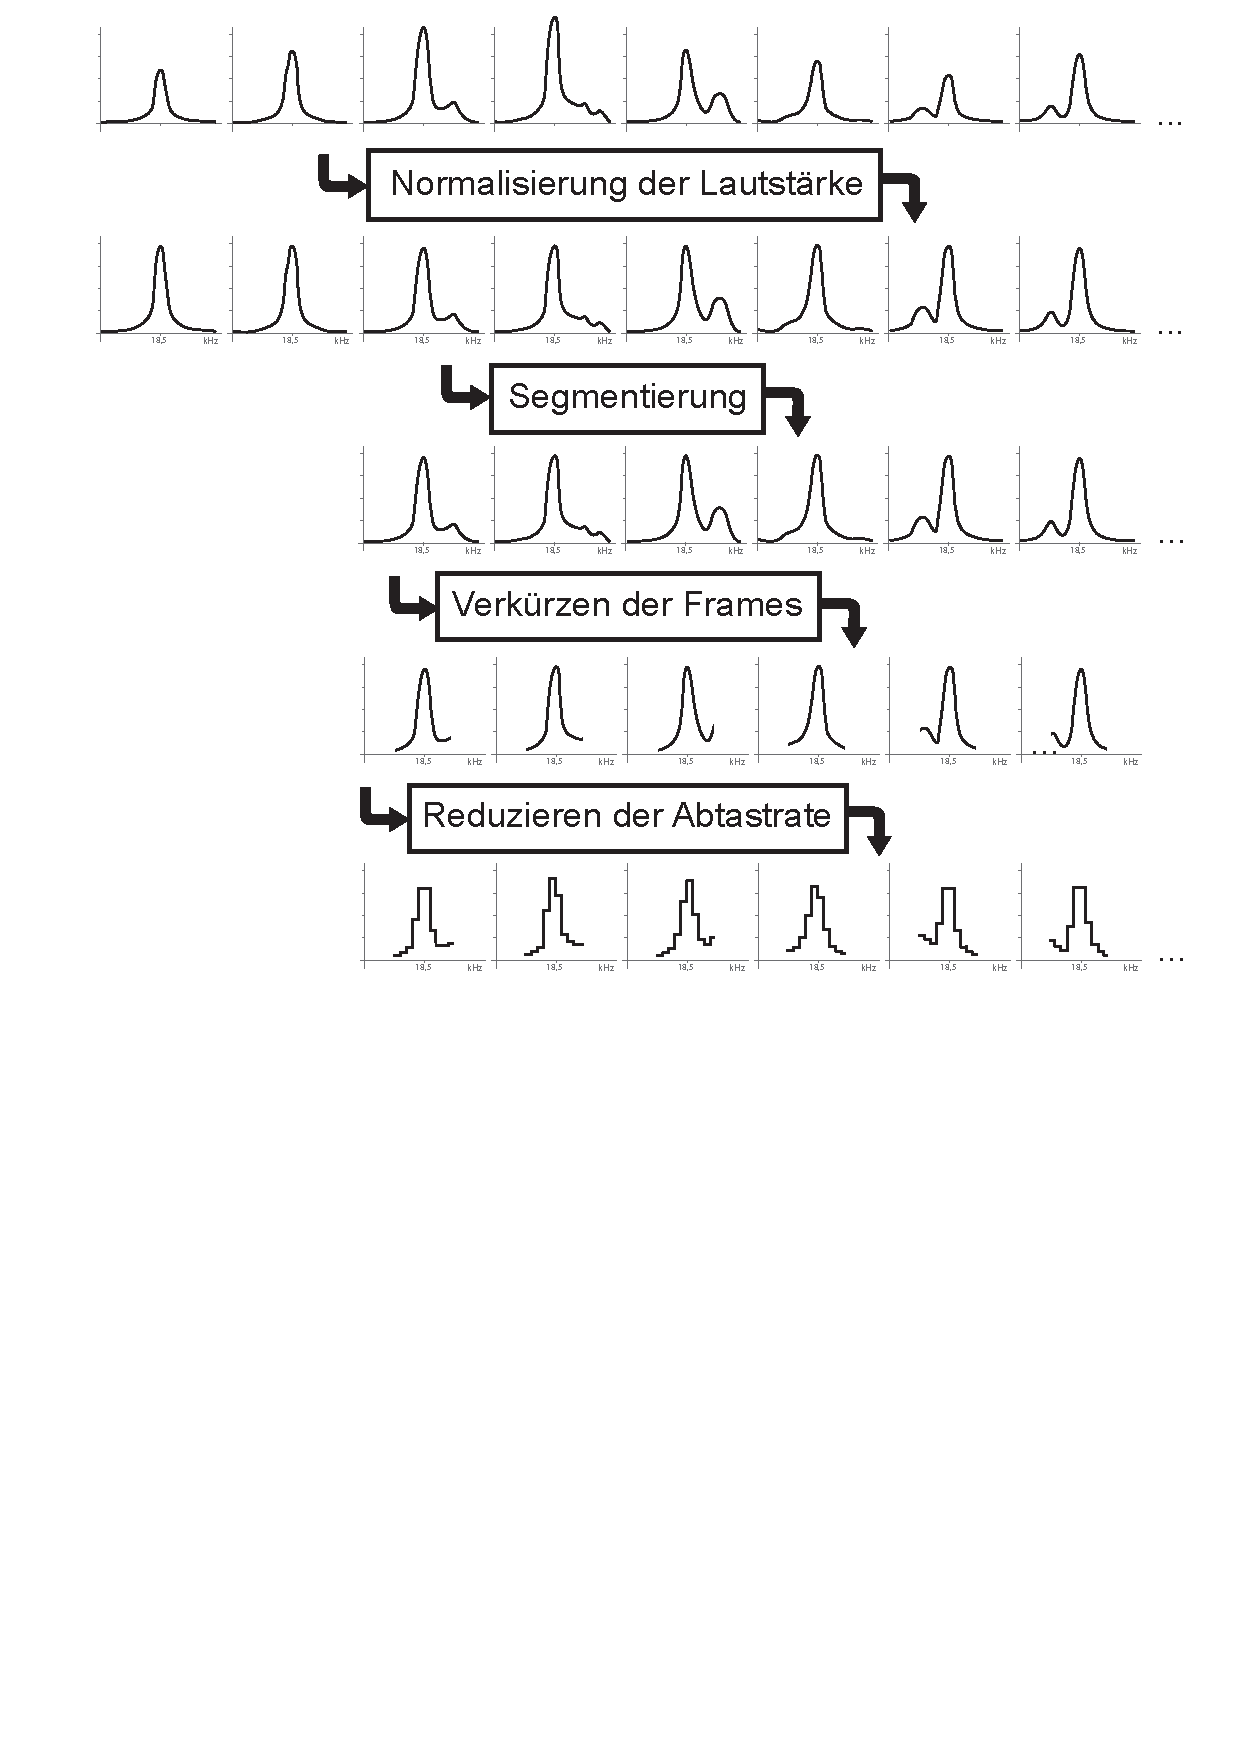
\includegraphics[width=0.9\textwidth]{kmeans/Vorverarbeitung.pdf}
\caption{Vorverarbeitung der Aufnahmen}
\label{fig:kMeansVorverarbeitung}
\end{figure*}

%Norm. -> Segmentierung -> Reduzieren der Datenmenge
Insgesamt ist erkennbar, dass bei den übrigen Gesten neben der Amplitude jeweils mindestens ein weiteres lokales Maximum existiert. Anhand dieser Maxima ist eine Unterscheidung vom Grundrauschen und somit auch eine Segmentierung der relevanten Frames aus einer Gestenaufnahme möglich.

Die Datenaufbereitung erfolgt in der in \autoref{fig:kMeansVorverarbeitung} dargestellten Reihenfolge. 
Zu Beginn wird eine Normalisierung der 
Lautstärke durchgeführt. Dazu werden alle Lautstärkewerte in jedem einzelnen Frame so um den gleichen Prozentsatz erhöht beziehungsweise verringert, dass die Amplitude jedes Frames einen vorher festgelegten Maximalwert annimmt. Dieser Schritt ist notwendig, da bei der verwendeten Hardware die Lautstärke der Aufnahmen stark schwankt.
%Im Anschluss daran werden die Frames einer Aufnahme so segmentiert, dass 
%sich der Beginn der Geste bei jeder Aufnahme an der gleichen Frame-Postion
%möglichst nur die Frames übrig bleiben, bei denen die Geste ausgeführt wird.

Im Anschluss daran erfolgt die Segmentierung der Gesten. Dabei werden aus den Aufnahmen die nicht relevanten Frames vor und nach Ausführung der eigentlichen Geste entfernt. Diese Frames bestehen nur aus dem Grundrauschen und enthalten daher keine Informationen, die für die weitere Klassifikation hilfreich sind.
% Diese bestehen eh nur aus Grundrauschen und sind daher für die weitere Klassifikation nicht weiter hilfreich / nicht nützlich. befindet.  
Für diesen Bearbeitungsschritt muss erkannt werden, zu welchem Zeitpunkt eine Geste ausgeführt wird. Dazu werden bei allen Frames die lokalen Maxima des Frequenzspektrums ermittelt, da sich bei Ausführung einer Geste zusätzliche lokale Maxima bilden.
Aus diesen lokalen Maxima wird anschließend der zweitgrößte Wert ermittelt. Der größte Wert wird nicht weiter verwendet, da sich dieser immer an der Stelle der Referenzfrequenz von 18,5 kHz befindet. 
Der Frame, bei dem der zweitgrößte Wert der lokalen Maxima am größten ist, wird nun als Bestandteil der Geste erkannt. 
Im folgenden Schritt werden die 24 Frames ermittelt, während denen die Geste ausgeführt wird. 
%Ausgehend von diesem Frame werden 24 Frames der gesamten 48 Frames beibehalten.
Dazu werden neben dem gefundenen Frame eine als Margin bezeichnete Anzahl von $m$ Frames davor sowie die $24-m-1$ nachfolgenden Frames beibehalten. Bei der Segmentierung ist die Wahl eines passenden Werts für $m$ sehr wichtig, damit die Geste vollständig erfasst wird. Ist $m$ zu klein, werden die Frames zu Beginn der Geste nicht gespeichert. Umgekehrt werden bei einem zu großen Wert für $m$ die Frames am Ende der Geste gelöscht. Eine Aufnahme hat nach diesem Vorverarbeitungsschritt grundsätzlich eine Länge von 24 Frames. Falls die Dauer der Geste unter 24 Frames liegt, ist in den restlichen hinteren Frames das Grundrauschen gespeichert.

Nach Abschluss der Segmentierung hat sich die Datenmenge durch die Beschränkung auf 24 Frames bereits von 3072 auf 1536 Dimensionen halbiert. Um das Ergebnis der Klassifikation zu optimieren, erfolgt eine weitere Reduzierung der Dimensionen. Dazu werden die ersten und letzten 24 Lautstärkewerte jedes Frames entfernt, da die zur Gestenerkennung relevanten Frequenzverschiebungen nur in den 8 Frequenzbereichen unterhalb und oberhalb der Referenzfrequenz von 18,5 kHz stattfinden. Somit verringert sich die Anzahl der Dimensionen auf 384. Zuletzt werden die nun vorhandenen Daten weiter reduziert, indem die Abtastrate innerhalb der einzelnen Frames mehrmals halbiert wird. Dazu werden je zwei aufeinanderfolgende Lautstärkewerte des Frames zu einem neuen Lautstärkewert zusammengefasst, der dem arithmetischen Mittel der beiden ursprünglichen Werte entspricht. Diese Halbierung wird pro Frame zweimal durchgeführt.
Insgesamt reduziert sich somit die Anzahl der Dimensionen pro Geste nach dem vollständigen Durchlaufen der Vorverarbeitung von ursprünglich 3072 auf 96 Dimensionen. 


Es zeigte sich, dass die Geste \ac{OT} nach der Datenaufbereitung nicht zuverlässig von den übrigen Gesten unterscheiden lässt. Aus diesem Grund wird die Klassifizierung dieser Geste nicht weiter verfolgt. Zusätzlich kann jedoch eine Bewegung von unten nach oben (Bottom-To-Top-One-Hand, im Folgenden kurz BTO) erkannt werden, die daher bei der weiteren Klassifikation ebenfalls berücksichtigt wird. Insgesamt werden vom Klassifikator die Gesten \ac{TBO}, BTO, \ac{SPO}, \ac{DPO} sowie das Hintergrundrauschen (\ac{BNS} und \ac{BNN}) unterstützt. Die beiden Klassen für das Hintergrundrauschen werden dabei zu einer Klasse zusammengefasst, es wird also nicht lauter und leiser Umgebung unterschieden. Es existiert daher nur eine Klasse für alle Aufnahmen, die keiner Geste entsprechen.

\subsubsection{Anpassung des Klassifikators}
Der Klassifikator wurde nur geringfügig angepasst.
In der Initialisierungsphase werden die Startpunkte der Cluster-Zentren nicht wie im ursprünglichen Algorithmus zufällig gewählt, sondern mithilfe des in \autoref{subsec:kMeansFunktionsweise} vorgestellten k-Means++ Algorithmus bestimmt.
Dadurch ergeben sich in der Regel eine schnellere Laufzeit in der Trainingsphase sowie bessere Ergebnisse bei der Klassifikation.
Die Trainingsphase läuft hingegen unverändert ab.
Weiterhin gilt eine Geste als nicht eindeutig bestimmt, wenn der Abstand zum zweitnächsten Cluster-Zentrum nicht mindestens um einen bestimmten Prozentsatz $p$ größer ist als der Abstand zum nächsten Zentrum. Es hat sich dabei herausgestellt, dass 10\% ein geeigneter Wert für $p$ ist.


Zur Bestimmung der Geste werden zwei verschiedene k-Means Klassifikatoren verwendet. Zu Beginn entscheidet der erste Klassifikator, ob es sich um die Geste \ac{SPO}, die Geste \ac{DPO} oder eine der anderen Gesten handelt.
%eine der Gesten \ac{SPO} oder \ac{DPO} handelt.
Falls weder die Geste \ac{SPO} noch die Geste \ac{DPO} erkannt wird, unterscheidet der zweite Klassifikator, ob es sich um die Geste \ac{TBO}, die Geste BTO oder das Hintergrundrauschen handelt. 
Während der Trainingsphase eines Klassifikators wird die Berechnung der Cluster-Zentren mehrmals hintereinander wiederholt. Dabei wird bei jeder so ermittelten Menge von Cluster-Zentren der Abstand der zwei nächsten Zentren berechnet. Als Klassifikator wird schließlich derjenige ausgewählt, bei dem dieser Abstand am größten ist.


\begin{figure*}[htbp]
    \centering
   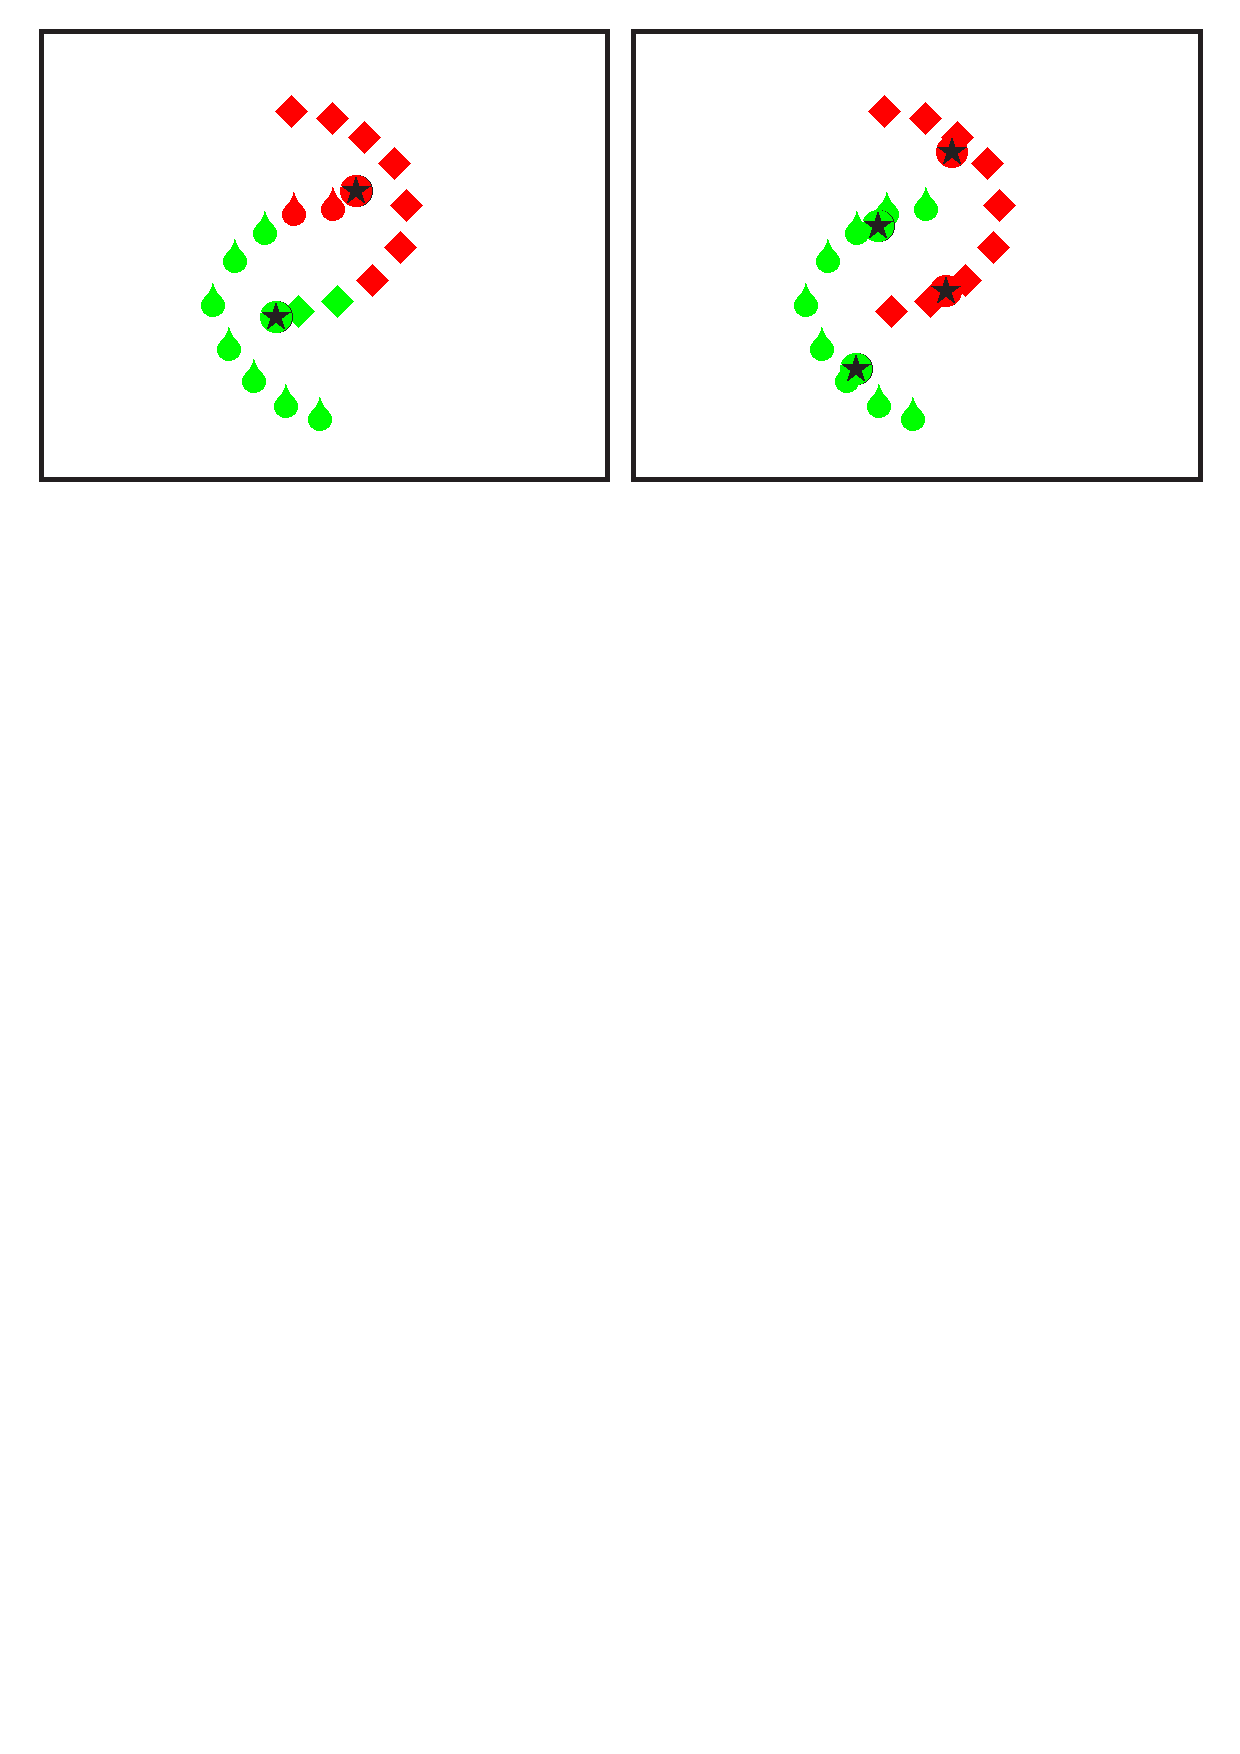
\includegraphics[width=.85\textwidth]{kmeans/kMeansWertK.pdf}
\caption{Klassifizierung mit k=2 (links) und k=4 (rechts)}
\label{fig:kMeansWertK}
\end{figure*}

Ansonsten wurden keine Veränderungen am Algorithmus vorgenommen.
Für die Qualität der Klassifikation ist weiterhin die Wahl eines geeigneten Werts für \emph{k} von Bedeutung. \autoref{fig:kMeansWertK} zeigt ein Beispiel, bei dem der k-Means Algorithmus für zwei Gruppen von Daten mit einem Wert von k = 2 ein sehr ungenaues Ergebnis liefert. Für k=4 funktioniert das Clustering sehr gut, da 
nun pro Gruppe je zwei Cluster-Zentren existieren.
Zur Gestenerkennung muss \emph{k} mindestens um eins größer sein als die Anzahl der Gesten (da mindestens eine Klasse für das Grundrauschen benötigt wird),
damit der Algorithmus in der Lage ist, die einzelnen Aufnahmen voneinander zu unterscheiden.  


Grundsätzlich gibt es zur Ermittlung der Anzahl an Clustern in einem Datensatz viele verschiedene Ansätze, etwa die Faustregel $k \approx \sqrt{n/2}$ \cite{WikipediaKMeansKValue}, wobei \emph{n} der Anzahl der Datenpunkte entspricht. Im Fall der hier beschriebenen Gestenerkennung kann der Wert für \emph{k} jedoch bereits grob abgeschätzt werden. 
Die untere Grenze ist wie bereits erwähnt um eins größer als die Anzahl der Gesten.
Als obere Grenze lässt sich grob der fünffache Wert der unteren Grenze abschätzen, da davon auszugehen ist, dass es nur wenige Variationsmöglichkeiten beim Ausführen einer Geste gibt.

%Nach der Lernphase ist es noch notwendig, dass den einzelnen Cluster-Zentren je eine Geste zugeordnet wird. Dazu wird ermittelt, welche Geste wie oft in die einzelnen Cluster-Zentren eingeordnet wird. Falls \emph{k} gleich dem oben genannten Minimalwert ist, reicht es aus, dem ersten Cluster die am häufigsten dort vorkommende Geste zuzuordnen, dem zweiten Cluster die häufigste vorkommende Geste der übrigen Gesten und so weiter.
%Somit ergibt sich der in 
%\autoref{lst:kmeans_zuordnung1}
%dargestellte Algorithmus.
%Als Ergebnis erhält man eine Menge von Zuordnungen von Cluster-Zentren zu Gesten. Die Anzahl dieser Zuordnungen entspricht der Anzahl der Gesten.
%
%\begin{lstlisting}[language=Python,caption={Pseudocode der Zuordnung von Cluster-Zentren zu Gesten, Variante 1},label={lst:kmeans_zuordnung1}]{lst:kmeans_zuordnung1}
%for Geste in alleGesten:
%    suche aus der Liste der Cluster das Cluster, zu dem die Geste am      häufigsten zugeordnet wird
%    speichere die Zuordnung des gefundenen Clusters zur Geste
%    entferne das gefundene Cluster aus der Liste
%\end{lstlisting}
%
%Ist \emph{k} größer als der Minimalwert, werden zuerst die \emph{k} Cluster, bei denen die Anzahl der am häufigsten zugeordneten Geste maximal ist, gemäß 
%\autoref{lst:kmeans_zuordnung1} durchlaufen und jedem dieser Cluster eine andere Geste zugeordnet. Anschließend wird jedem übrigen Cluster die Geste zugeordnet, die am häufigsten in das Cluster eingeordnet wurde.
%Insgesamt ergibt sich der in \autoref{lst:kmeans_zuordnung2} dargestellte Algorithmus.  Als Ergebnis erhält man eine Menge von Zuordnungen von Clustern zu Gesten. Die Anzahl dieser Zuordnungen entspricht der Anzahl an Clustern.
%
%\begin{lstlisting}[language=Python,caption={Pseudocode der Zuordnung von Cluster-Zentren zu Gesten, Variante 2},label={lst:kmeans_zuordnung2}]{lst:kmeans_zuordnung2}
%Erstelle eine Zuordnung von Clustern zu Gesten mit dem Algorithmus aus Quelltext 4.1
%Erstelle eine Cluster-Liste, die alle noch nicht zugeordneten Cluster       enthält
%for Cluster in alleCluster:
%    suche aus der Liste der Gesten die Geste, die am häufigsten zu dem Cluster zugeordnet wird
%    speichere Zuordnung von Cluster zu gefundener Geste
%\end{lstlisting}
%
%Die in \autoref{lst:kmeans_zuordnung1} und \autoref{lst:kmeans_zuordnung2} dargestellten Algorithmen arbeiten
%zuverlässig, wenn die Gesten -- bis auf wenige Ausnahmen -- eindeutig einem Cluster zugeordnet werden können. Ist dies nicht der Fall, kann keine akzeptable Gestenerkennung realisiert werden und die Vorverarbeitung und/oder der Wert von \emph{k} sollte angepasst werden.


\subsubsection{Implementierung} \label{subsubsec:kMeansImpl}
Die Implementierung erfolgt in der Programmiersprache Python unter Verwendung der Bibliothek skikit-learn (Version 0.14) \cite{sklearn}. Diese Bibliothek verwendet den beschriebenen k-Means Algorithmus von Lloyd. Außerdem bietet sie noch die Möglichkeit, dass die Startpunkte der Cluster-Zentren nicht wie im ursprünglichen Algorithmus vorgesehen zufällig gewählt, sondern stattdessen mit dem k-Means++ Algorithmus bestimmt werden. Zusätzlich können noch weitere 
%kleine 
Einstellungen vorgenommen werden, um den Klassifikator für den jeweiligen Anwendungsfall  zu optimieren. Dazu gehört beispielsweise eine Beschränkung der Iterationen beim Lernen auf einen bestimmten Maximalwert.
Die Komplexität im ungünstigsten Fall liegt bei $O(n^{(k+2)/p})$ \cite{sklearn.kmeans, kMeansHowSlow}, wobei $n$ der Anzahl der Trainingsdaten und $p$ der Anzahl der Dimensionen entspricht.

Das entwickelte Klassifikationssystem ist in das in \autoref{sec:app} beschriebene Rahmenprogramm eingebettet. Nach dem Öffnen der grafischen Benutzeroberfläche können die -- in Form von Cluster-Zentren gespeicherten --  Einstellungen zur Klassifikation geladen werden. Ein Training des Klassifikators ist im Experten-Modus möglich, der über den zweiten Tab der GUI aufgerufen werden kann. Die vier unterstützten Gesten sind an die in in \autoref{tab:kMeansKeyGestures} dargestellten Aktionen gebunden, die in einem zu Demonstrationszwecken angezeigten QT-Label durchgeführt werden.
%Windows-Tastaturkommandos gebunden, sodass nach dem Ausführen einer Geste das in \autoref{tab:kMeansKeyGestures} angegebene Tastaturkommando angestoßen wird.

\begin{table}[h]
\centering
\begin{tabular}{|p{0.17\textwidth}|p{0.24\textwidth}|}
\hline
 \textbf{Geste} & \textbf{Tastaturkommando} \\
 \hline
  \ac{TBO} & nach unten scrollen \\
 \hline
  BTO & nach oben scrollen \\
 \hline
  \ac{SPO} & Schriftart ändern \\
 \hline
  \ac{DPO} & Zum Textanfang oder Textende springen \\
 \hline
\end{tabular}
\caption[Tastaturkommandos, die den Gesten zugeordnet sind]{Tastaturkommandos, die den Gesten zugeordnet sind}
\label{tab:kMeansKeyGestures}
\end{table}



\subsubsection{Evaluation}
Es hat sich gezeigt, dass die Klassifikation für $k$ gleich der Anzahl der zu bestimmenden Klassen die besten Ergebnisse liefert.  
Nicht vom Klassifikator unterstützt und daher nicht bei der Evaluation berücksichtigt werden die Gesten \ac{RLO}, \ac{OT} und \ac{RO}. Zum Testen der Erkennungsrate wurden die übrigen Gesten sowie die eigene Geste BTO jeweils 20 mal ausgeführt. Für das Hintergrundrauschen wurden typische Bewegungen während der Arbeit am Laptop ausgeführt, etwa Mausbewegungen oder Tippen auf der Tastatur. Die Ergebnisse der Klassifikation sind in  \autoref{matrix_kMeansEvaluation} als Wahrheitsmatrix dargestellt. Die Reihenfolge der Gesten ist dabei (von links nach rechts beziehungsweise von oben nach unten) \ac{TBO}, BTO, \ac{SPO}, \ac{DPO} und das Grundrauschen.

\begin{center}
\begin{equation}
\label{matrix_kMeansEvaluation}
\begin{pmatrix}
19 & 0 & 0 & 0 & 1\\
0 & 17 & 1 & 0 & 2\\
2 & 4 & 14 & 0 & 0\\
1 & 1 & 2 & 16 & 0\\
0 & 0 & 0 & 0 & 20
\end{pmatrix}
\end{equation}
\end{center}


\begin{table}[h]
\centering
\begin{tabular}{|p{0.17\textwidth}|c|}
\hline
 \textbf{Geste} & \textbf{Erkennungsrate} \\
 \hline
  \ac{TBO} & 95\% \\
 \hline
  BTO & 85\% \\
 \hline
  \ac{SPO} & 70\% \\
 \hline
  DPO & 80\% \\
 \hline
  \ac{BNS} \& \ac{BNN} (Hintergrund\-rauschen) & 100\%\\
 \hline
\end{tabular}
\caption[Erkennungsraten beim k-Means Klassifikator]{Erkennungsraten beim k-Means Klassifikator}
\label{tab:kMeansEvaluation}
\end{table}

%Bei welchen Parameter-Werten werden die besten Ergebnisse erzielt?
%Stark von Hardware abhängig
%Geschwindigkeit, Training VS Erkennung

\subsection{Fazit}
%Wie gut funktioniert die Erkennung? Welche Gesten werden gut, welche schlecht erkannt? Ausblick auf potentielle weiterführende Arbeiten.

Mit dem implementierten k-Means Klassifikationssystem können die Gesten \ac{TBO}, BTO, \ac{SPO} und \ac{DPO} in Echtzeit erkannt und voneinander unterschieden werden.
%Die Geste \ac{RLO} wird nicht vom Klassifikator unterstützt, da sie sich nicht deutlich genug von der Geste \ac{SPO} unterscheidet. Weiterhin kann die Geste \ac{RO} nicht erkannt werden, da sie keine erkennbaren Unterschiede zum Grundrauschen aufweist.
Nicht bei der Klassifikation berücksichtigt wurden die Gesten \ac{RLO}, \ac{OT} und \ac{RO}. Als zusätzliche Geste wird die Bewegung einer Hand von unten nach oben (BTO) unterstützt.
Am besten erkannt werden die Gesten \ac{TBO} und BTO mit einer Erkennungsrate von 95 beziehungsweise 85 Prozent. Weniger gut erkannt werden die Gesten \ac{SPO} (70 Prozent) und \ac{DPO} (80 Prozent). 

Insgesamt liefert der Klassifikator gute Ergebnisse, eine weitere Optimierung der Erkennungsrate ist jedoch 
für den praktischen Einsatz wünschenswert.
%Die beste Erkennungsrate  
%Das Ziel war, die Anwendung auf jedem Rechner mit Mikrofon und Lautsprecher ausführen zu können. Durch die starke Abhängigkeit von der Hardware ist dies nur eingeschränkt möglich. 
Nicht betrachtet wurde die Möglichkeit, neben den vorgegebenen Gesten eigene Gesten zu definieren und zu erkennen. Eine denkbare Erweiterung ist es, als zusätzliches Eingabegerät die an Notebooks standardmäßig vorhandene Kamera bei der Gestenerkennung zu berücksichtigen. Dies ist insbesondere für Gesten interessant, die zu einer ähnlichen Frequenzverschiebung führen und daher anhand des Audiosignals nicht zuverlässig unterschieden werden können. 

% Wie viel Einfluss hat die Hardware? Wie mit schwierigen Hardwarebedingungen wie Lausprecher nach unten umgehen?
% Weitere, nicht fest vorgegebene Gesten
% Möglichkeit, die sehr ähnlichen Gesten und zu unterscheiden?
% Verbesserung der Erkennung durch Verwendung von mehreren Klassifikatoren bzw. weiterer Eingaben (wie Kamera)